\chapter{Marco Teórico}
\thispagestyle{empty}

\section{Redes neuronales}
El término de red neuronal fué acuñado por \citet{McCulloch1943}
para describir el primer modelo computacional de una red neuronal, sin embargo el modelo que planteaban no tenía la capacidad de aprender, carecía de un algoritmo de aprendizaje. Aunque el modelo planteado por \citeauthor{McCulloch1943} no sea lo suficientemente preciso para describir el funcionamiento del cerebro, sentó las bases para el estudio de las neuronas como modelos computacionales.


El trabajo de \citet{Rosenblatt1957}, pese a no ser el primero, contribuyó a la popularización de la primera generación de RNA: los perceptrones. \citeauthor{Rosenblatt1957} diseñó el algoritmo de aprendizaje del perceptrón con un concepto llamado ``correción mediante propagación hacia atrás del error'' (\textit{back-propagating error correction}), concepto que se sigue utilizando hasta hoy. \citep{Rumelhart1986}.

Las RNs son buenos aproxiadores de funciones (\citeauthor{Hornik1989}, \citeyear{Hornik1989}; \citeauthor{Cybenko1989}, \citeyear{Cybenko1989})

% \subsection{Las redes neuronales y sus características}

% Gradiente

% La técnica de optimización (El descenso del gradiente)

% La función de pérdida (error cuadráico medio), con la técnica de optimización se trata de minimizar el error por medio del ajuste de los pesos de la red.

% Bakpropagation

% El aprendizaje consiste en combinar dos cosas. El algortimo de backpropagation con una técnica de optimización.

% El entrenamiento de una red neuronal se realiza por medio de un algoritmo denominado \textit{backpropagation} (propagación de errores hacia atras), termino acuñado por \citet{Rumelhart1986}. Este algoritmo permite a la red neuronal ajustar los parámetros $\theta_i$ por medio del cálculo del gradiente de error. Esto quiere decir que, nos permite saber como varía el error conforme varían los parámetros de la red.  


% El algoritmo de \textit{bagpropagation} se encarga del informarnos en que sentido se han de modificar los parámetros de la red, mientras que la técnica de optimización realiza el ajuste de los parámetros.


% \subsection{La redes neuronales como aproximadores de funciones}


% \subsection{Parámetros e hiperparámetros de una red neuronal}
% \subsection{Precisión de un modelo de red neuronal}

\subsection{Redes neuronales informadas por la física}
El aprendizaje automático ha provocado un cambio fundamental en el método científico. Tradicionalmente, la investigación científica ha girado en torno a la teoría y la experimentación: una mano diseña una teoría bien definida y luego la refina continuamente utilizando datos experimentales y los analiza para hacer nuevas predicciones.

Pero hoy, con los rápidos avances en el campo del aprendizaje automático y cantidades cada vez mayores de datos científicos, los enfoques basados en datos se han vuelto cada vez más populares. Aquí no se requiere una teoría existente y, en su lugar, se puede usar un algoritmo de aprendizaje automático para analizar un problema científico utilizando solo datos.

Veamos una forma en que el aprendizaje automático se puede utilizar para la investigación científica. Imagine que nos dan algunos puntos de datos experimentales que provienen de algún fenómeno físico desconocido, por ejemplo, los puntos naranjas en la animación a continuación.

Una tarea científica común es encontrar un modelo que sea capaz de predecir con precisión nuevas mediciones experimentales a partir de estos datos.
\begin{figure}[htbp]
    \caption{Ejemplo de una red neuronal que ajusta un modelo a algunos datos experimentales\sep}
    \label{figure:redNeuronal01}
    \begin{center}
        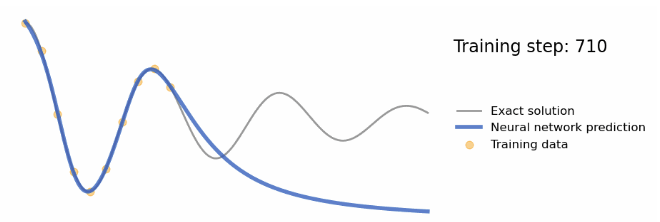
\includegraphics[width=0.75\textwidth]{img/redNeuronal01.png}
    \end{center}
        \begin{tablenotes}
            \item {{\fontsize{10pt}{ \baselineskip}\selectfont \textit{Nota.} Tomado de \url{https://benmoseley.blog/my-research/so-what-is-a-physics-informed-neural-network/} }}
        \end{tablenotes}
\end{figure}

Una forma popular de hacer esto usando el aprendizaje automático es usar una red neuronal. Dada la ubicación de un punto de datos como entrada (indicado como x), se puede usar una red neuronal para generar una predicción de su valor (indicado tucomo ), como se muestra en la figura \ref{figure:redNeuronal02}:
\begin{figure}[htbp]
    \caption{Esquema de una red neuronal\sep}
    \label{figure:redNeuronal02}
    \begin{center}
        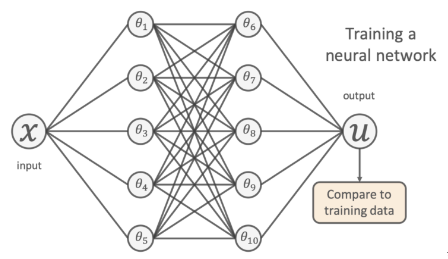
\includegraphics[width=0.75\textwidth]{img/redNeuronal02.png}
    \end{center}
        \begin{tablenotes}
            \item {{\fontsize{10pt}{ \baselineskip}\selectfont \textit{Nota.} Tomado de \url{https://benmoseley.blog/my-research/so-what-is-a-physics-informed-neural-network/}}}
        \end{tablenotes}
\end{figure}

Para aprender un modelo, tratamos de ajustar los parámetros libres de la red (indicados por la \ thetas en la figura anterior) para que las predicciones de la red coincidan estrechamente con los datos experimentales disponibles. Esto generalmente se hace minimizando el error cuadrático medio entre sus predicciones y los puntos de entrenamiento;
\begin{equation}
    min \frac{1}{N} \sum^N_i \left(u_{NN}(x_i;\theta) - u_{true}(x_i)\right)^2
\end{equation}
En la figure \ref{figure:redNeuronal01} se muestra el resultado de entrenar una red neuronal de este tipo utilizando los datos experimentales anteriores.

El problema es que usar un enfoque puramente basado en datos como este puede tener desventajas significativas. Eche un vistazo a los valores reales del proceso físico desconocido utilizado para generar los datos experimentales en la figura \ref{figure:redNeuronal01} (línea gris).

Puede ver que, si bien la red neuronal modela con precisión el proceso físico en la vecindad de los datos experimentales, no logra generalizar a partir de estos datos de entrenamiento. Confiando únicamente en los datos, se podría argumentar que realmente no ha “comprendido” el problema científico.

Si quisieramos solucionar el siguiente problema físico:
\begin{equation}
    m \frac{d^2 u}{d x^2} + u\frac{du}{dx} + ku = 0
\end{equation}
Donde $m$ es la masa del oscilador, $\mu$ es el coeficiente de fricción y $k$ es la constante del resorte.

Al usar el esquema de RN de la figura \ref{figure:digrama de flujo PINN} podemos ver que la pérdida física adicional en la función de pérdida intenta asegurar  que la solución aprendida por la red sea consistente con la física conocida, mediante la siguiente función de pérdida para entrenar la red.
\begin{equation}
    min \frac{1}{N}\sum^N_i \left(u_{NN}()x_i; \theta) - u_{true}(x_i)\right)^2 + \frac{1}{M}\sum^M_j\left(\left[m\frac{d^2}{dx^2}+\mu\frac{d}{dx}+k\right]u_{NN}(x_j;\theta)\right)^2
\end{equation}

\begin{figure}[htbp]
    \caption{Diagrama de flujo del algoritmo PINN\sep}
    \label{figure:digrama de flujo PINN}
    \begin{center}
        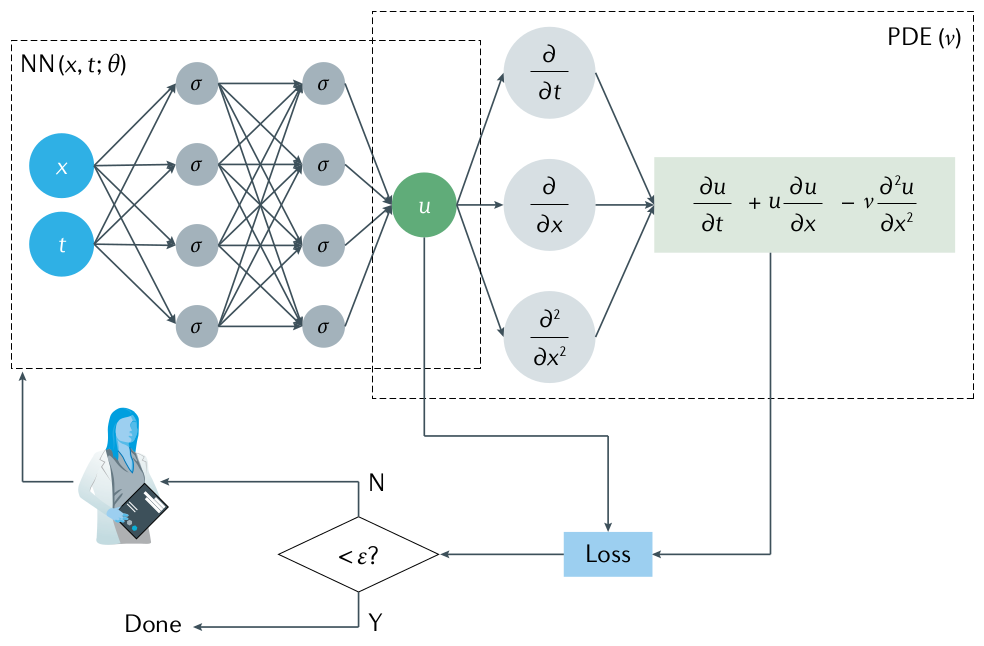
\includegraphics[width=0.75\textwidth]{img/pinns01.png}
    \end{center}
        \begin{tablenotes}
            \item {{\fontsize{10pt}{ \baselineskip}\selectfont \textit{Nota.} Tomado de ``Physics-informed machine learning'' (p. 425), por \citeauthor{Karniadakis2021}, \citeyear{Karniadakis2021}, \textit{Nature Reviews Physics, 3.} }}
        \end{tablenotes}
\end{figure}
Los resultados cuando entrenamos la red informada por la física podemos verlo en la figura \ref{figure:redNeuronal03}
\begin{figure}[htbp]
    \caption{Red neuronal informada por la física que aprende a modelar un oscilador armónico\sep}
    \label{figure:redNeuronal03}
    \begin{center}
        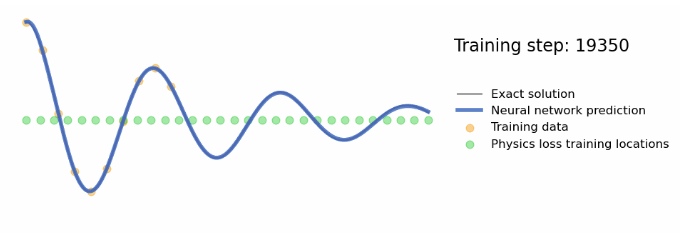
\includegraphics[width=0.75\textwidth]{img/redNeuronal03.png}
    \end{center}
        \begin{tablenotes}
            \item {{\fontsize{10pt}{ \baselineskip}\selectfont \textit{Nota.} Tomado de \url{https://benmoseley.blog/my-research/so-what-is-a-physics-informed-neural-network/}}}
        \end{tablenotes}
\end{figure}

% \section{Ecuación de onda}
% \subsection{La ecuación de onda y sus caracterísiticas}
% \subsection{Solución numérica de la ecuación de onda y sus características}


% \section{Construcción de una red neuronal informada por la física}




% La redes neuronales (RN) son la unidad funcional del aprendizaje profundo que imita el comportamiento del cerebro humano para resolver problemas complejos basados en datos. Los datos de entradas se procesan a través de diferentes capas de neuronas artificiales apiladas para producir el resultado deseado. Diversas investigaciones(\cite{Breen2019}; \cite{Raissi2017}; \cite{Nguyen2021}; \cite{Scellier2021}; \cite{Iten2018}) .

% Las entradas, que vienen a ser los {\it features}, ingresan al cuerpo de la ''neurona`` multiplicandose cada uno por unos pesos, realizando una combinación lineal de los pesos con los {\it features} $u_i = \sum_j = w_{ij} y_j$. Seguidamente se define una función $y_i = f(u_i)$, la cual tiene que garantizar la no linealidad.





% \begin{figure}[htbp]
%     \caption{Red neurona artificial y biológica\sep}
%     \label{fig:red neuronal y biologica}
%     \begin{center}
%         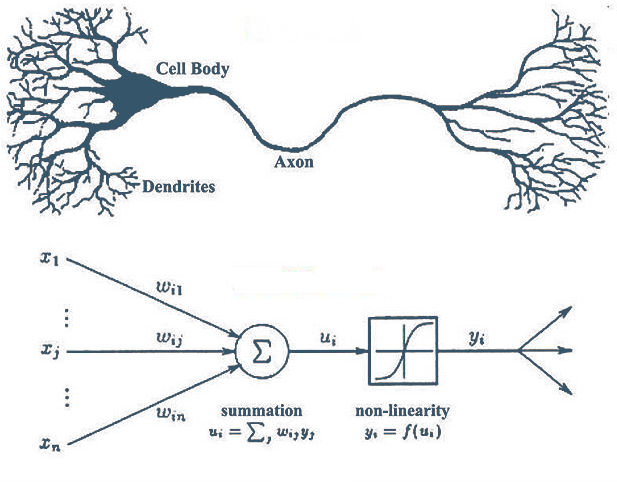
\includegraphics[width=0.6\textwidth]{img/red_neuronal.png}
%     \end{center}
%         % \begin{tablenotes}
%         %     \item {{\fontsize{10pt}{ \baselineskip}\selectfont \textit{Nota.} }}
%         % \end{tablenotes}
% \end{figure}

% 
% \section{Objetivos generales}
% Caracterizar los recursos hídricos e identificar las zonas vulnerables en el ámbito del Proyecto Especial Tambo Ccaracocha mediante el modelamiento geoespacial y presentar alternativas de aprovechamiento de los recursos hídricos.

% \section{Objetivos específicos}
% % [leftmargin=1em]
% \begin{itemize}
%     \item Determinar la oferta y demanda hídrica en el ámbito de influencia del Proyecto Especial Tambo-Ccaracocha. 
%     \item Presentar alternativas de proyectos, para contribuir a la segurar el afianzamiento hídrico para el valle de Ica. 
%     \item Generar una base de datos geoespacial, para caracterizar e identificar el grado de vulnerabilidad en el ámbito del Proyecto Tambo Ccaracocha.
%     \item Desarrollar el modelo geoespacial para identificación del grado de vulnerabilidad en el ámbito del Proyecto. 
% \end{itemize}

